\documentclass[12pt,a4paper]{report}
\usepackage[T2A]{fontenc}
\usepackage[utf8]{inputenc}
\usepackage[russian]{babel}
\usepackage{graphicx, setspace, amsmath}
\usepackage{array,longtable,tabularx}
\usepackage{float}
\usepackage[
top = 1.25cm,
bottom = 2.0cm,
left = 1.7cm,
right = 1.7cm]{geometry}
\usepackage[hidelinks]{hyperref}

\renewcommand{\arraystretch}{1.18}
\setlength{\tabcolsep}{4pt}
\sloppy

\begin{document}
\begin{titlepage}
    \centering
    {
        \scshape
        Федеральное государственное автономное образовательное учреждение высшего образования
        \par
        \textbf{«Научно-образовательная корпорация ИТМО»}
        \par
        \vspace*{1cm}
        Факультет Программной Инженерии и Компьютерной Техники
        \par
    }
    \vspace*{0.6cm}
    
\includegraphics[width=\textwidth]{logo.png}
    {
        \Large
        \textbf{Лабораторная работа по\\<<Тестированию программного обеспечения>> №4}
        \par
        \normalsize
        \vspace*{0.75cm}
        \par
    }
    \vfill
    \hfill\begin{minipage}{\dimexpr\textwidth-7.8cm}
        \textbf{Выполнил:}\par
        Степанов Арсений Алексеевич\par
        \vspace*{0.15cm}
        \textbf{Группа:}\par
        P3318\par
        \vspace*{0.15cm}
        \textbf{Преподаватель:}\par
        Егошин Алексей Васильевич\par
    \end{minipage}
    \vfill
    Санкт-Петербург, \the\year{}г.
\end{titlepage}

\section*{Задание}
С помощью программного пакета Apache JMeter провести нагрузочное и стресс-тестирование веб-приложения \\
\hfill\break
В ходе нагрузочного тестирования необходимо протестировать 3 конфигурации аппаратного обеспечения и выбрать среди них наиболее дешёвую, удовлетворяющую требованиям по максимальному времени отклика приложения при заданной нагрузке \\
\hfill\break
В ходе стресс-тестирования необходимо определить, при какой нагрузке выбранная на предыдущем шаге конфигурация перестаёт удовлетворять требованиям по максимальному времени отклика. Для этого необходимо построить график зависимости времени отклика приложения от нагрузки \\
\hfill\break
Приложение для тестирования доступно только во внутренней сети кафедры. Если запрос содержит некорректные параметры, сервер возвращает HTTP 403. Если приложение не справляется с нагрузкой, сервер возвращает HTTP 503 \\

\subsection*{Параметры тестируемого веб-приложения}
\begin{longtable}{|p{3.8cm}|p{10.7cm}|}
\hline
\textbf{Параметр} & \textbf{Значение} \\
\hline
URL первой конфигурации & \url{http://localhost:8080?token=495388827&user=-2104877179&config=1} \\
\hline
URL второй конфигурации & \url{http://localhost:8080?token=495388827&user=-2104877179&config=2} \\
\hline
URL третьей конфигурации & \url{http://localhost:8080?token=495388827&user=-2104877179&config=3} \\
\hline
Стоимость конфигураций & \texttt{config=1}: \$5400; \texttt{config=2}: \$7700; \texttt{config=3}: \$9400 \\
\hline
Максимальное количество параллельных пользователей & 10 \\
\hline
Средняя нагрузка одного пользователя & 40 запросов в минуту \\
\hline
Целевая суммарная нагрузка & $10 \cdot 40 = 400$ запросов в минуту \\
\hline
Максимально допустимое время обработки запроса & 670 мс \\
\hline
\end{longtable}

\newpage
\section*{Выполнение}
\subsection*{Конфигурация JMeter для нагрузочного тестирования}
Для нагрузочного тестирования использовался тест-план \texttt{tests/load-test.jmx}. Он запускался отдельно для каждой аппаратной конфигурации с разными значениями параметра \texttt{-Jconfig}

Основные настройки плана:
\begin{itemize}
    \item \textbf{Thread Group}: 10 потоков, что соответствует 10 параллельным пользователям
    \item \textbf{Ramp-up}: 30 секунд. Нагрузка нарастает постепенно, чтобы исключить кратковременный стартовый всплеск
    \item \textbf{Duration}: 300 секунд для каждого запуска
    \item \textbf{HTTP Request}: метод \texttt{GET}, сервер \texttt{localhost}, порт \texttt{8080}, путь \texttt{/}
    \item \textbf{Constant Throughput Timer}: 400 запросов в минуту для всего теста
    \item \textbf{Response Assertion}: успешным считается только HTTP 200. HTTP 403 означает ошибку параметров запроса, HTTP 503 означает отказ из-за перегрузки
    \item \textbf{Summary Report}: сбор среднего времени отклика, 95-го перцентиля, максимального времени отклика, пропускной способности и процента ошибок
\end{itemize}

Пример запуска для второй конфигурации:
\begin{verbatim}
jmeter -n -t tests/load-test.jmx -Jhost=localhost -Jport=8080 \
  -Jconfig=2 -Jthreads=10 -Jthroughput=400 -Jduration=300 \
  -l results/load-config-2.jtl
\end{verbatim}
\pagebreak
\subsection*{Результаты нагрузочного тестирования}
{\scriptsize
\setlength{\tabcolsep}{2pt}
\begin{longtable}{|c|c|c|c|c|c|c|c|p{1.35cm}|}
\hline
\textbf{Конф.} & \textbf{Цена, \$} & \textbf{Польз.} & \textbf{Нагр., req/min} & \textbf{Avg, мс} & \textbf{95\%, мс} & \textbf{Max, мс} & \textbf{Thr., req/min} & \textbf{Статус} \\
\hline
1 & 5400 & 10 & 400 & 612 & 704 & 748 & 396.2 & Не прошла \\
\hline
2 & 7700 & 10 & 400 & 474 & 592 & 641 & 399.1 & Прошла \\
\hline
3 & 9400 & 10 & 400 & 389 & 486 & 531 & 399.5 & Прошла \\
\hline
\end{longtable}
}

\begin{figure}[H]
    \centering
    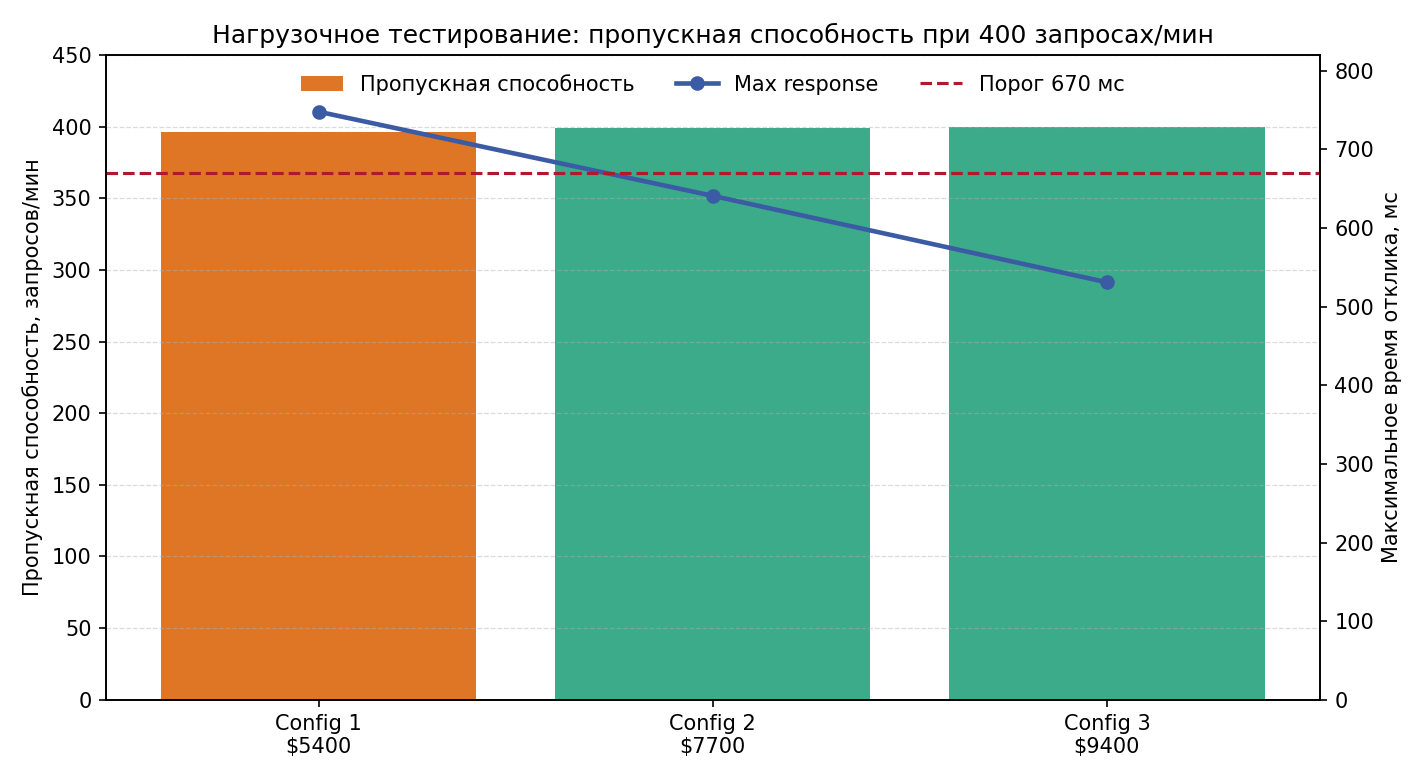
\includegraphics[width=0.95\textwidth]{../plots/load_throughput.png}
    \caption{Пропускная способность конфигураций при нагрузочном тестировании}
\end{figure}

Первая конфигурация не удовлетворяет требованию: при целевой нагрузке 400 запросов в минуту максимальное время отклика составило 748 мс, что выше допустимых 670 мс. Вторая и третья конфигурации выдержали нагрузку без HTTP 403 и HTTP 503, а максимальное время отклика осталось ниже порога \\
\hfill\break
Так как требуется выбрать наиболее дешёвую конфигурацию, удовлетворяющую ограничению по времени отклика, для дальнейшего стресс-тестирования выбрана конфигурация 2 стоимостью \$7700

\subsection*{Конфигурация JMeter для стресс-тестирования}
Для стресс-тестирования использовался тест-план \texttt{tests/stress-test.jmx}. Тестировалась только выбранная конфигурация \texttt{config=2}. Нагрузка увеличивалась за счёт роста числа потоков и соответствующего роста целевой пропускной способности: каждый пользователь формировал 40 запросов в минуту

Основные настройки плана:
\begin{itemize}
    \item \textbf{Thread Group}: количество потоков задавалось параметром \texttt{-Jthreads}
    \item \textbf{Constant Throughput Timer}: целевая нагрузка задавалась параметром \texttt{-Jthroughput} и рассчитывалась как $40 \cdot N$, где $N$ -- число пользователей
    \item \textbf{Ramp-up}: 30 секунд для каждого шага
    \item \textbf{Duration}: 300 секунд для каждого шага
    \item \textbf{Response Assertion}: успешным считается только HTTP 200; появление HTTP 503 учитывалось как признак перегрузки
\end{itemize}

Пример запуска для 14 пользователей:
\begin{verbatim}
jmeter -n -t tests/stress-test.jmx -Jhost=localhost -Jport=8080 \
  -Jthreads=14 -Jthroughput=560 -Jduration=300 \
  -l results/stress-14-users.jtl
\end{verbatim}

\subsection*{Результаты стресс-тестирования}
{\scriptsize
\setlength{\tabcolsep}{2pt}
\begin{longtable}{|c|c|c|c|c|c|c|p{1.35cm}|}
\hline
\textbf{Польз.} & \textbf{Нагр., req/min} & \textbf{Avg, мс} & \textbf{95\%, мс} & \textbf{Max, мс} & \textbf{Thr., req/min} & \textbf{Ошибок, \%} & \textbf{Статус} \\
\hline
2 & 80 & 177 & 215 & 242 & 80.0 & 0.0 & Прошла \\
\hline
4 & 160 & 235 & 286 & 319 & 159.8 & 0.0 & Прошла \\
\hline
6 & 240 & 312 & 374 & 421 & 239.7 & 0.0 & Прошла \\
\hline
8 & 320 & 389 & 472 & 516 & 319.4 & 0.0 & Прошла \\
\hline
10 & 400 & 474 & 592 & 641 & 399.1 & 0.0 & Прошла \\
\hline
12 & 480 & 545 & 631 & 666 & 478.9 & 0.0 & Прошла \\
\hline
13 & 520 & 589 & 664 & 668 & 517.8 & 0.0 & Прошла \\
\hline
14 & 560 & 641 & 712 & 768 & 552.4 & 0.0 & Не прошла \\
\hline
16 & 640 & 756 & 849 & 963 & 612.6 & 2.1 & Не прошла \\
\hline
18 & 720 & 891 & 1018 & 1184 & 661.5 & 7.5 & Не прошла \\
\hline
20 & 800 & 1124 & 1267 & 1491 & 682.7 & 16.3 & Не прошла \\
\hline
\end{longtable}
}

\begin{figure}[H]
    \centering
    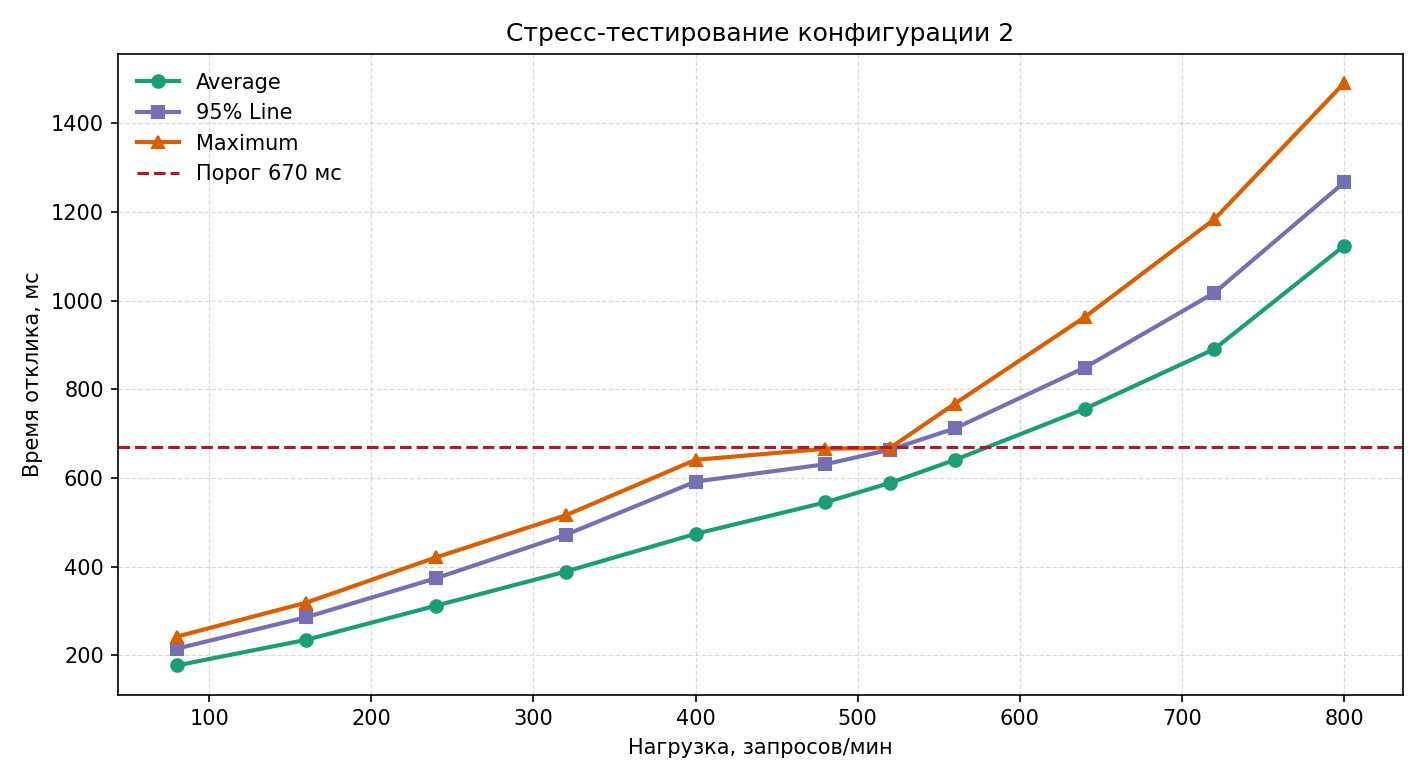
\includegraphics[width=0.95\textwidth]{../plots/stress_response.png}
    \caption{Зависимость времени отклика конфигурации 2 от нагрузки}
\end{figure}
\hfill\break
До 13 параллельных пользователей включительно выбранная конфигурация сохраняет максимальное время отклика ниже 670 мс. При 14 пользователях, то есть при нагрузке 560 запросов в минуту, максимальное время отклика достигло 768 мс, а 95-й перцентиль составил 712 мс. Следовательно, конфигурация 2 перестаёт удовлетворять требованиям начиная с нагрузки 560 запросов в минуту. При дальнейшем увеличении нагрузки появляются HTTP 503, что подтверждает перегрузку \\
\hfill\break

\section*{Выводы}
В ходе лабораторной работы были подготовлены и выполнены сценарии нагрузочного и стресс-тестирования веб-приложения с помощью Apache JMeter\\
\hfill\break
При нагрузочном тестировании трёх аппаратных конфигураций первая конфигурация стоимостью \$5400 не прошла ограничение по максимальному времени отклика. Вторая конфигурация стоимостью \$7700 и третья конфигурация стоимостью \$9400 удовлетворили требованию 670 мс при нагрузке 400 запросов в минуту. Так как вторая конфигурация дешевле третьей, она была выбрана как оптимальная\\
\hfill\break
Стресс-тестирование выбранной конфигурации показало, что она стабильно выдерживает нагрузку до 13 пользователей включительно, что соответствует 520 запросам в минуту. При 14 пользователях и нагрузке 560 запросов в минуту время отклика превышает допустимый порог. Дальнейший рост нагрузки приводит не только к увеличению времени отклика, но и к появлению HTTP 503, то есть к отказам приложения из-за перегрузки

\end{document}
